\subsection{Conceptos del Modelo de Negocio}

En esta sección tiene como finalidad explicar conceptos clave para la formación del modelo de negocio basados en el libro "Generación de modelos de negocio"\cite{modeloNegocio}

\subsection{Modelo de negocio: }

Se refiere a la forma en que una empresa crea, entrega y captura valor. Es una representación simplificada de cómo una organización planea generar ingresos y obtener beneficios. Según el libro "Business Model Generation" de Alexander Osterwalder y Yves Pigneur, un modelo de negocio puede definirse como "la lógica mediante la cual una organización crea, entrega y captura valor" \cite{modeloNegocio}

\subsection{Modelo canva}
El Modelo Canvas es una herramienta visual utilizada para desarrollar o innovar modelos de negocio de una empresa de manera clara y sencilla. Fue propuesto por Alexander Osterwalder en su libro "Business Model Generation" y se ha convertido en un estándar para emprendedores, startups y empresas que buscan estructurar sus ideas o revisar sus estrategias.
\begin{itemize}
    \item Segmentos de mercado: Define los diferentes grupos de personas o empresas que la organización busca atender o servir. Aquí se identifican los clientes objetivo.
    \item Propuesta de valor: Explica el valor añadido que se ofrece a los clientes. ¿Qué problemas resuelve tu producto o servicio? ¿Por qué los clientes elegirían tu oferta sobre la de la competencia?
    \item Canales: Indica cómo la empresa llegará a sus clientes, desde la comunicación hasta la distribución del producto o servicio. Pueden ser tanto canales físicos como digitales.
    \item Relación con los clientes: Describe el tipo de interacción que la empresa establece con cada segmento de clientes. ¿Es una relación personalizada, automatizada, de autoservicio, etc.?
    \item Flujos de ingresos: Detalla cómo la empresa generará ingresos a partir de su propuesta de valor. Esto puede incluir ventas directas, suscripciones, publicidad, comisiones, entre otros.
    \item Recursos clave: Describe los activos más importantes necesarios para que el modelo de negocio funcione, como recursos humanos, financieros, físicos o intelectuales.
    \item Actividades clave: Son las acciones estratégicas que la empresa debe realizar para ejecutar su modelo de negocio. Pueden ser la producción, el marketing, la investigación y desarrollo, etc.
    \item Socios clave: Muestra las alianzas y asociaciones necesarias para hacer funcionar el modelo. Esto incluye proveedores, socios estratégicos y otras empresas o entidades que aporten valor.
    \item Estructura de costos: Expone los costos más significativos asociados a la operación del negocio, como los costos fijos y variables, inversión en tecnología, sueldos, etc.
\end{itemize}

A continuación en la figura %%\ref{plantillaModeloCanva}
presenta la estructura del modelo canva , usado para ilustrar el modelo de negocio.
\begin{adjustbox}{
    center,
    caption=[{Modelo Canva}]{\centering Modelo Canva. Fuente:(Sitio web: Modelo de negocio Canvas: Qué es y cómo usarlo, según Ylse Roa, 2023)},
    label={plantillaModeloCanva},
    nofloat=figure}

    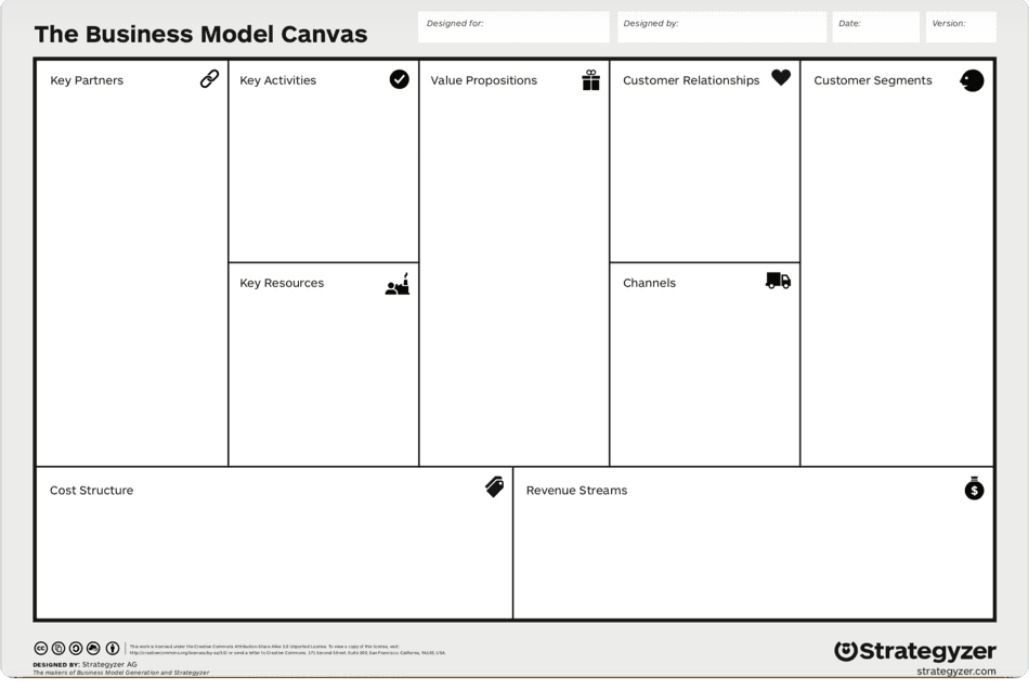
\includegraphics[scale=0.4]{Content/Images/modelo canva plantilla.jpeg}

\end{adjustbox}